%%%%%%%%%%%%%%%%%%%%%%%%%%%%%%%%%%%%%%%%%%%%%%%%%%%%%%%
% % Lines starting with % are comments, which are ignored.
% % This is a handy way of indicating the date and version of
% % your document, to wit:
% %
% % LaTeX sample file
% % Modified March, 2002
% %
%%%%%%%%%%%%%%%%%%%%%%%%%%%%%%%%%%%%%%%%%%%%%%%%%%%%%%%
\DocumentMetadata{
  % PDF standards: ONE key whose value is a comma-separated list --
  % UA-2 (accessibility) plus A-4f (archival; the archival companion of
  % UA-2). Do NOT use separate pdfstandard=... keys: with ordinary
  % key-value parsing only the last one takes effect.
  pdfstandard={UA-2,A-4f},
  lang=en-US,
  tagging=on,
  tagging-setup={
    math/setup=mathml-SE
  }
}

\documentclass[12pt]{exam}
% worksheet-macros.tex -- shared package setup for worksheet-template.tex.
%
% NOTE ON PATHS: every template in this repository is stored one level up
% from where it is compiled (see README.md). All relative \input paths
% below are resolved against the folder the document is compiled in,
% which sits one directory above this file.

% --- Math ------------------------------------------------------------
% amsmath: equation environments and numbering
% amsfonts: \mathbb etc.  |  mathrsfs: \mathfrak  |  stmaryrd: extra symbols
\usepackage{amsmath}
\usepackage{amsfonts}
\usepackage{mathrsfs}
\usepackage{stmaryrd}

% --- Layout and glyphs ------------------------------------------------
% float: [H] float placement (stop floats where you put them)
% fontspec: Unicode/OpenType fonts (compile with XeLaTeX or LuaLaTeX)
% emoji: emoji glyphs in the text
\usepackage{float}
\usepackage{fontspec}
\usepackage{emoji}

% --- Typography --------------------------------------------------------
% Atkinson Hyperlegible as the document-wide sans serif (sfdefault):
% a high-legibility face that is easier to read for students with
% dyslexia or low vision.
\usepackage[sfdefault]{atkinson}

% --- Colors -------------------------------------------------------------
% dvipsnames: extended named color palette (the Accessible* colors in
%   lecture-macros.tex are built on it);
% table: \rowcolors / \cellcolor for shading worksheet tables.
% NOTE: xcolor may only be loaded ONCE per document -- a second
% \usepackage{xcolor} with different options is a fatal "Option clash"
% error, so ALL of its options are listed here.
\usepackage[dvipsnames,table]{xcolor}

% --- Multimedia ---------------------------------------------------------
% animate: embeds audio/video (and legacy Flash) media in the worksheet.
\usepackage{animate}

% --- Bibliography --------------------------------------------------------
% biblatex (biber backend): citations and a reference list for worksheets.
\usepackage[
  backend=biber,
  style=alphabetic,
  url=true,
  doi=true,
  isbn=true,
  backref=true
]{biblatex}

% --- Links ---------------------------------------------------------------
% hyperref makes every \ref/citation/URL clickable in the PDF.
% Link colors must satisfy WCAG 1.4.3 (>= 4.5:1 contrast on white):
%   blue = 8.6:1, green!40!black = 7.2:1.
% (The old cyan/magenta values measured 1.25:1 / 3.1:1 and failed.)
\usepackage{hyperref}
\hypersetup{
  colorlinks=true,
  linkcolor=blue,
  filecolor=blue,
  urlcolor=green!40!black,
}

% --- Shared course macros ------------------------------------------------
% Root macros.tex: math shorthands used across all course documents
% (\RR, \NN, \ZZ, \QQ, \grad, \curl, \tr, \der, \pder, ...).
\newcommand{\RR}{\mathbb{R}}
\newcommand{\NN}{\mathbb{N}}
\newcommand{\ZZ}{\mathbb{Z}}
\newcommand{\QQ}{\mathbb{Q}}
\newcommand{\vv}{\vec{v}}
\newcommand{\ww}{\vec{w}}
\newcommand{\xx}{\vec{x}}
\newcommand{\yy}{\vec{y}}
\newcommand{\zz}{\vec{z}}
\newcommand{\uu}{\vec{u}}
\newcommand{\basis}[1]{\vec{e_{#1}}}
\newcommand{\id}{\mathrm{id}}
\newcommand{\CC}{\mathbb{C}}
\renewcommand{\div}{\operatorname{div}}
\newcommand{\grad}{\operatorname{grad}}
\newcommand{\curl}{\operatorname{curl}}
\newcommand{\tr}{\operatorname{tr}}
\newcommand{\der}[2]{\dfrac{d #1}{d #2}}
\newcommand{\pder}[3][]{\dfrac{\partial^{#1} #2}{\partial #3}}


% % Title and author(s)
%%%%%%%%%%%%%%%%%%%%%%%%%%%%%%%%%%%%%%%%%%%%%%%%%%%%%%%
\title{Worksheet 8 - Continuity and Differentiability}
\author{MATH 1271}
\date{10/01/2026}
%%%%%%%%%%%%%%%%%%%%%%%%%%%%%%%%%%%%%%%%%%%%%%%%%%%%%%%
% %
% % The next command allows your in import encapsulated
% % postscript files, .epsf or .eps files, which
% % contain vector graphic image data.
% %
%%%%%%%%%%%%%%%%%%%%%%%%%%%%%%%%%%%%%%%%%%%%%%%%%%%%%%%
% %   The first thanks indicates your affiliation
% %
% %  Just the name here.
% %
% % Your mailing address goes at the end.
% %
% % \thanks is also how you indicate grant support
% %
%%%%%%%%%%%%%%%%%%%%%%%%%%%%%%%%%%%%%%%%%%%%%%%%%%%%%%%

%%%%%%%%%%%%%%%%%%%%%%%%%%%%%%%%%%%%%%%%%%%%%%%%%%%%%%%
% $ The next command ensures the margins are 1 inch on
% % all sides.
% %
%%%%%%%%%%%%%%%%%%%%%%%%%%%%%%%%%%%%%%%%%%%%%%%%%%%%%%%
\begin{document}
\newpage
\maketitle
\begin{enumerate}


\item Consider the function $f(x)$ graphed below. You may assume that $f(2)=-2.5$. 

\begin{center}
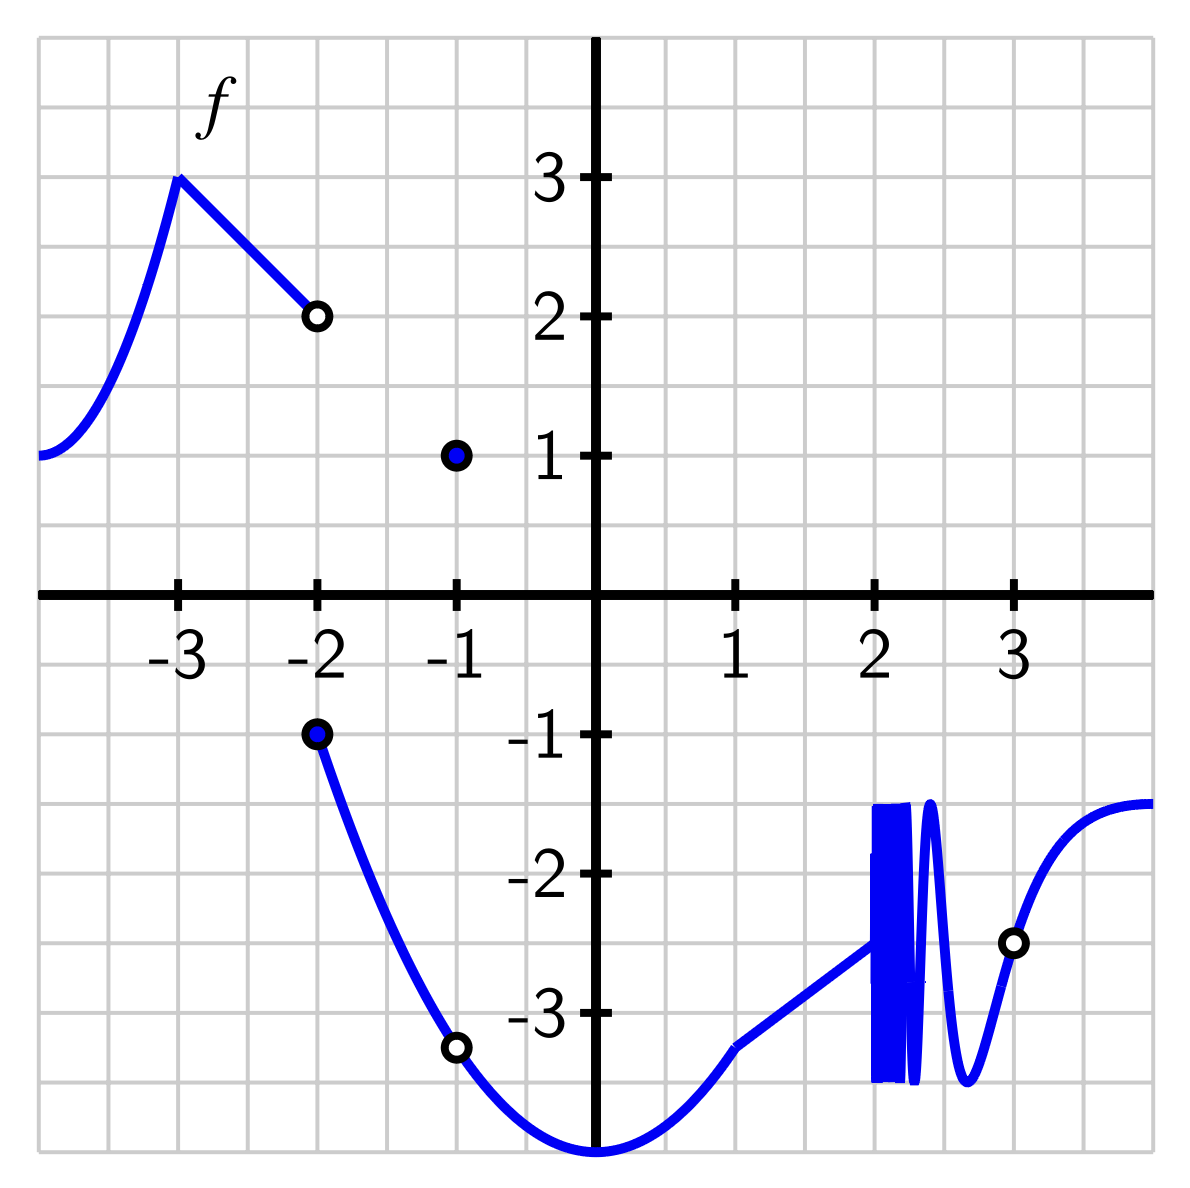
\includegraphics[scale=0.33]{wkst8img}
\end{center}

\begin{enumerate}

\item At which values of $a$ does $\displaystyle\lim_{x\to a}f(x)$ not exist?

\vfill

\item At which values of $a$ is $f(a)$ not defined?

\vfill

\item At which values of $a$ does $f$ have a limit (i.e., $\displaystyle\lim_{x\to a}f(x)$ exists), but $\displaystyle\lim_{x\to a}f(x)\neq f(a)$?

\vfill

\item Based on your reasoning above, state all values of $a$ for which $f$ is \emph{not} continuous at $x=a$.

\vfill

\item State all values of $a$ for which $f$ is \emph{not} differentiable at $x=a$. (Give a reason for each of your answers.)

\vfill

\end{enumerate}

\newpage



\item 

\begin{enumerate}

\item Consider the following piecewise-defined function:
$$f(x)=\begin{cases} 3x+8 &\text{if $x\leq 0$}\\[3pt] \frac{2}{3}x+\frac{7}{3} &\text{if $0<x\leq 1$}\\[3pt] 4-x &\text{if $x>1$}\end{cases}$$

\begin{enumerate}

\item Compute $f(0)$ and $f(1)$.

\vspace{1.75in}

\item For each of the values $a=0$ and $a=1$, compute $\displaystyle\lim_{x\to a^-}f(x)$ and $\displaystyle\lim_{x\to a^+}f(x)$.

\vspace{2.25in}

\item Based on your work above, is $f$ continuous at $a=0$? How about at $a=1$? (Why?)

\vspace{1.75in}

\end{enumerate}

\newpage

\item Consider the following piecewise-defined function, where $a$ and $b$ are constants:
$$g(x)=\begin{cases} a+bx &\text{if $x<2$}\\[3pt] 5 &\text{if $x=2$}\\[3pt] x^2-bx+a &\text{if $x>2$}\end{cases}$$

\begin{enumerate}

\item In terms of $a$ and $b$, what is $\displaystyle\lim_{x\to 2^-}g(x)$?

\vspace{1in}

\item In terms of $a$ and $b$, what is $\displaystyle\lim_{x\to 2^+}g(x)$?

\vspace{1in}

\item What is $g(2)$?

\vspace{1in}

\item What values of $a$ and $b$ make $g(x)$ continuous at $x=2$?

\vspace{1in}

\end{enumerate}

\item Determine the value of $b$ that makes the function
$$h(x)=\begin{cases} b-x &\text{if $x<5$}\\[3pt] -x^2+6x-6 &\text{if $x\geq 5$}\end{cases}$$
continuous at $x=5$. Clearly explain how you got your answer. 

\vfill

\end{enumerate}
\newpage

\item We'll use the topics we learned this lecture to explicitly determine the structure of the linear approximation $f(x) \approx a + b(x - x_0) $ of a function $f(x)$ around $x = x_0$. We'll show that $a = f(x_0),$ and $ b=f'(x_0)$.

  Throughout this exercise we'll assume that the real numbers $a,b,c$ satisfy:
  \begin{equation}
    \label{eq:best_quad}
    \lim_{x \rightarrow x_0} \dfrac{f(x) - (a + b(x-x_0) )}{(x - x_0)} = 0
  \end{equation}
  and that $f(x)$ is differentiable at $x = x_0$.

  We'll first show that $a = f(x_0)$.
  \begin{enumerate}
    \item Assume instead that:
      \begin{equation}
        \label{eq:const_lim}
        \lim_{x \rightarrow x_0} (f(x) - (a + b(x - x_0) ) = 0
      \end{equation}
      and use that, along with the continuity of $f(x)$ at $x = x_0$,
      to show that $a = f(x_0)$.
      \vfill
    \item How can we use our assumed limit equation \autoref{eq:best_quad}
      to imply \autoref{eq:const_lim}?
      \vfill
  \end{enumerate}
  \newpage

  We'll now show that $b = f'(x_0)$.
  \begin{enumerate}
    \item Now use \autoref{eq:best_quad} 
      and that $f(x)$ is differentiable at $x = x_0$ to manipulate the limit and determine that $b = f'(x_0)$. (The limit definition of the derivative will be useful here.)
      \vfill
  \end{enumerate}
  
  We could do a similar derivation of the \textit{quadratic} approximation,
  but that unfortunately relies on a stronger version of the Mean Value Theorem. I'd be happy to discuss that in office hours, however!


\end{enumerate}

% Most people don't use these, so they are "commented out"
% by starting the lines with a "%"
%\begin{keywords}
%   \LaTeX, typesetting
%\end{keywords}

%\begin{AMS}
%   50C60, 18C25
%\end{AMS}

%%%%%%%%%%%%%%%%%%%%%%
% % Here is the start of the Text
%%%%%%%%%%%%%%%%%%%%%%
\end{document}
